% additional options: [seceqn,secthm,crcready,onecolumn]
\documentclass[ida]{iosart2x}

%% Packages
\usepackage{dcolumn}
\usepackage{amsmath}
\usepackage{graphicx}

\usepackage{algorithmicx,algorithm}
\usepackage{algpseudocode} 
\usepackage{subfigure}
\usepackage{multirow}
\usepackage{booktabs}
\usepackage{subfigure}
%\usepackage{endnotes}

%% Definitions
\newcolumntype{d}[1]{D{.}{.}{#1}}

%% Article Info
\firstpage{1}
\lastpage{16}
\volume{1}
\pubyear{2020}

\begin{document}

\begin{frontmatter} % The preamble begins here.

%
%\pretitle{Pretitle}
\title{Oversampling algorithm of imbalanced classification using DBSCAN and gaussian distribution}

%\author{Yinuo Xiao\inst{1}}
%\institute{Harbin Institute of Technology,}
%\email{xiaoyinuo@hit.edu.cn}}

\author[A]{\inits{F.}\fnms{Yinuo} \snm{Xiao}\ead[label=e1]{xiaoyinuo@hit.edu.cn}},
and
\author[B]{\inits{S.}\fnms{Rui} \snm{Li}\ead[label=e2]{LiRui.HITstu@gmail.com}}
\runningauthor{Y. Xiao et al.}{Oversampling algorithm of imbalanced classification using DBSCAN and gaussian distribution}

\address[A]{Harbin Institute of Technology \printead[presep={\\}]{e1}}
\address[B]{Harbin Institute of Technology \printead[presep={\\}]{e2}}

\begin{abstract}
  Classification over imbalanced data, which often leads to poor prediction ability for 
  minority class(es), is a challenging tasks in machine learning.
  Many algorithms, including SMOTE and its derivatives, 
  have been proposed to
  solve this problem by a means of rebanlancing the data distribution via oversampling. However, 
  the effects of these algorithms are still unsatisfactory. This paper proposes
  new oversampling algorithm by integrating DBSCAN and gaussian distribution into oversampling.  
  First, minority data points(data samples) are
  divided into core, borderline and noise points by DBSCAN. 
  Second, the total number of oversampling data points is
  assigned for different kinds of data points. Third, 
  we synthetic new points using gaussian distribution.
  % Therefore we propose new oversampling methods called ODG and MC-ODG, In these methods,
  % DBSCAN and gaussian distribution were applied to generate new sample points. 
  The experiment results
  show that our methods have high prediction ability compared with existing methods.
\end{abstract}

\begin{keyword}
\kwd{imbalance data}
\kwd{oversampling}
\kwd{DBSCAN}
\kwd{Gaussian distribution}
\end{keyword}
\end{frontmatter}




\section{Introduction}
%指出什么是不平衡数据集
Imbalanced data \cite{2004Editorial} refers to datasets that have an uneven 
amount of data between different classes. 
We assume that the majority class is negative class and 
the minority class is positive class in binary classification.

%不平衡数据处理的重要性,现在典型方法中存在的问题
The actual demand shows the importance and difficulty of learning on imbalanced datasets.
The imbalance occurs in many fields, such as medical 
diagnosis \cite{2013Computational,2019Electrocardiogram} and fault detection \cite{2018Imbalanced}.
In these cases ill samples and fault samples are minority samples.
%Although the sample size of minority class is small, 
We tend to be interested in minority samples because minority class contains more value. 
The disease samples need to be predicted more accurately than the normal samples, 
and the cost of misjudging fault samples is much higher than misjudging normal samples.
The difficulty %in solving imbalanced problems 
lies in the fact that existing machine 
learning models skew the prediction results towards 
majority class in the process of prediction \cite{Victoria2013An}, then 
the minority class cannot be classified correctly \cite{2016A}. 
Therefore, More advanced algorithms need to 
be proposed to improve the ability to predict minority class.

%现有的处理不平衡数据集的方法
The methods dealing with imbalance can be roughly
divided into two types: algorithm-level \cite{2007Highcost-sensitive} and data-level \cite{2002SMOTE}.
Algorithm-based approaches include BalanceCascade \cite{2019Class}, Adaboost, 
XGBoost \cite{Chen_2016}, etc. 
Algorithm-based methods are limited 
to a single type of classifier \cite{2020Combined} and 
cannot be extended to general machine learning models.
Data-level methods perform data preprocessing to reduce the imbalance ratio, Then 
the data can be processed effectively.
Data-level methods are generally divided into undersampling \cite{2015Undersampled} 
and oversampling \cite{2002SMOTE}. 
undersampling decreases the number of majority samples, %the price is losing part of the information, 
while oversampling enhances minority class by introducing new samples \cite{2010A}.
In our work, oversampling is used to preprocess the data.

%介绍基于数据的smote方法
%这里详细介绍了基于SMOTE算法的缺点,后面可以稍微省略一部分,后面需要展开讨论不同种SMOTE方法。
% Data-level methods address the imbalance by changing the data distributions and can be 
% applied with general mechine learning methods, such as SMOTE.
SMOTE is a classic oversampling algorithm,
%SMOTE is an improved method based on the random oversampling algorithm, 
SMOTE realizes changing the data distributions by randomly generating new sample 
on the line of minority points.
Numerous modifications of SMOTE algorithm have been proposed, such as
Borderline-SMOTE \cite{2005Borderline}, ADASYN \cite{2008ADASYN}, etc. 
However, SMOTE and its derivatives have their weaknesses,
they are susceptible to noise points and are difficult to deal with
 overlapping data distributions.
The generated minority points and majority points are easily covered, 
which affects the separating hyperplane of the classifier. 
In addition, $SMOTE$ methods can't handle
clusters of data. SMOTE is unable to capture the cluster distributions
if the monority sample points are distributed in clusters.
% Therefore, we could use 
% cluster methods.
% Clustering algorithm\cite{2011Data} divides the same set of data into multiple sets, 
% and the data in each set is similar. We can use
% clustering algorithms
% and dividing the data into multiple clusters, and then oversample data in each cluster.
Furthermore,
the method of syntheticing new points by SMOTE is difficult to 
maintain the original data distributions \cite{2008DATA},
After using $SMOTE$, 
the data distributions of minority sample points may change,
which will affect the prediction progress.


 %二分类和多分类
 SMOTE and its derivatives are also poor in multiple classification problems \cite{2020Combined}. 
 The relationship between two classes is relatively simple,
but in multiclassification problems, the relationship 
between classes becomes much more complex \cite{2017Relevance}.
When oversampling new points near the boundaries of multiple classes, 
creating overlapping data distributions \cite{Jierui2013Overlapping} is hard to avoid.
The existing methods to deal with multiclassification include transforming 
the problem into binary classification problems(OVO) \cite{articlemulti} or 
dividing the problem into one to many problems(OVA).
But processing two classes separately(OVO) will ignore the rest classes' information.
Treating one class as a minority class and the rest as a majority class(OVA)
cannot capture the relationship between majority classes effectively.
%Compared to other algorithm, MC-CCR algorithm can address multi-classification problems effectively.

%给出聚类算法
% If minority sample points are distributed in clusters, we could use 
% cluster methods.
% Clustering algorithm\cite{2011Data} divides the same set of data into multiple sets, 
% and the data in each set is similar. We can use
% clustering algorithms
% and divide the data into multiple clusters and oversample data in each cluster. There are many kinds of clustering algorithms, 
% among which the most famous one is K-MEANS\cite{2007K} algorithm.
% However, K-MEANS algorithm is a distance-based algorithm. 
% When there are irregular clusters, K-MEANS algorithm is difficult to handle, 
% meanwhile the parameter K is difficult to set. Therefore, 
% We use DBSCAN\cite{2013Mining} algorithm based on density.

%提出新的方法
Our work proposes new oversampling methods, which overcome above methods' drawbacks.
we proposed ODG(oversampling using DBSCAN and gaussian distribution) and MC-ODG
(multiclassification oversampling using DBSCAN and gaussian) algorithms 
for binary and multiple classification.
The proposed algorithms can solve the above problems, such as noise interference and oversampling. 
The generated points can keep the original data distributions.
% The ODG algorithm can be adaptive to determine how to 
% generate new sample points and how many sample points are generated around what kinds of points.
The new algorithms apply DBSCAN clustering method and gaussian
distribution to fit the data.
%注意单词的使用
The experimental results show that our algorithms are superior 
to the existing algorithms on different metrics.

%总结贡献
To summarize, our work makes the following contributions.
\begin{itemize}
  \item ODG is an oversampling method that can effectively process clustered data.
  \item We explain the influence of noise data points on the oversampling process and ODG shows how to deal with noise data points.
  \item ODG preserves the original data distributions after oversampling.
  \item ODG is suitable for binary classification, and its extension MC-ODG is suitable for multiclassification problems.
\end{itemize}

%文章组织
The paper is organized as follow. The next section introduces 
related works. Section 3 introduces our ODG and MC-ODG 
algorithms in details, 
and gives the specific flow of the algorithms and the corresponding complexity analysis.
In section 4, we introduce comparative experiments based on different models, 
and give the analysis and results of our experiments. Section 5 gives the summary and our future works.


\section{Related works}
This section provides required knowledge for our algorithms and some related oversampling methods.
\subsection{Clustering methods}

%\vspace{-0.1cm}
\textbf{Clustering} algorithm is to find groups of similar data, and each group of similar data forms a cluster.
There may be multiple clusters in a single minority class data, 
we need to use clustering algorithm to identify multiple clusters
 and then process each of them.The most famous clustering methods include distance-based K-MEANS algorithm and density-based DBSCAN algorithm.
K-MEANS algorithm is relatively simple, but this algorithm must determine the number of clusters K.
Meanwhile, compared with density-based DBSCAN algorithm, K-MEANS cannot find clusters with various shapes.
DBSCAN defines a cluster as the largest set of points
 connected by density and can find clusters of arbitrary shape. After the whole process,
  DBSCAN classifies minority points into core points,
  borderline points and noise points.
 Given the parameters $eps$ and $min\_pts$, we will get three kinds of points. 
 Core points have no less than
  $min\_pts$ points within $eps$ range. 
  Borderline points refer to the points that were partitioned into a cluster after DBSCAN,
  but not belong to core points. After the DBSCAN algorithm, The points that were not divided into any cluster are 
  defined as noise points.
The core points can best represent the distribution of the corresponding cluster, 
therefore we can use the distribution of the core points to generate data.
DBSCAN has been used for generating new points, such as DBSMOTE \cite{2012DBSMOTE} and
DSMOTE \cite{2019Over}, but these methods failed to escape the SMOTE limitation in 
the method of systneticing new samples and they did not use the distribution of minority class data.

\subsection{Related oversampling methods}

\textbf{Oversampling} balances the distribution of data 
by generating new data samples without losing information.
%这里着重介绍各个方法的细节,缺点之前已经详细介绍了
The fundamental idea of SMOTE is to generate new samples by interpolation between minority class samples \cite{2018SMOTE}.
Specifically, for a certain sample $x_i$, one of the K nearest neighbors is randomly selected as $x_i ^{'}$.
Use the Eq. \ref{equation14} to generate a new sample $x_{new}$. $\epsilon \in [0,1]$ is a random number.
\begin{equation}
  \label{equation14}
  x_{new}=x_i+(x_i-x_i^{'})\times \epsilon
\end{equation}ness of SMOTE,
% Using the algorithm of SMOTE, Generating new sample points inside the minority sample points is easy, 
% but new points are far from the classification surface, which has little influence on the classification prediction.
 SMOTE algorithm is easily affected by noise.
When noise data is present
, the new syntheticed samples may overlap with majority class samples.
Borderline-SMOTE \cite{2005Borderline} is based on SMOTE, this algorithm classifies
the minority samples into three types, 
$noise$, $danger$ and $safe$.
All the K nearest neighbors of the $noise$ points are majority points, 
more than half of the K nearest neighbors 
of the $danger$ points are majority points, 
and all of K nearest neighbors of $safe$ points are minority points.
Borderline-SMOTE uses $danger$ points to generate new samples.
To a certain extent Borderline-SMOTE reduced the negative effect of noise and overlapping data distribution.
ADASYN \cite{2008ADASYN} is an adaptive composite sampling method, 
a mechanism is used to determine how many samples need to be synthesized for each minority sample.
In general, for a minority sample, more majority points in its K nearest neighbors, 
the more minority points will be generated near this point.
There are also methods conbined oversampling and undersampling, such as SMOTE+ENN \cite{2019Electrocardiogram},
This method first deleted the majority points of which all of K nearest neighbors are minority points,
then use SMOTE to generate new samples.

% The way of generating new data in SMOTE is too simple, 
% Simply generating data on the line does not effectively preserve the original data distribution\cite{2017CCR,2020Combined}.
% In addition, for the problem of multiple classification, 
% methods based on SMOTE could not make use of the relationship between multiple classes during the process of 
% generation and expected effect cannot be achieved.
CCR \cite{2017CCR} and MC-CCR \cite{2020Combined} algorithms are oversampling algorithms based on $energy$,
In these methods, a spherical region is drawn at the center of each minority sample point. 
The spherical region is constantly expanding, when meeting a majority point the $energy$ is reduced.
When the $energy$ is exhausted, the region will no longer extend.
New data points are randomly generated inside the spherical region. 
The number of generated data is inversely proportional to the radius of the spherical region.
In addition, this method also proposed cleaning process, 
the majority points inside the spherical area will be shifted out to reduce overlapping.
But the CCR approach also has its drawbacks. In the process of generating data points,
the CCR method generates data randomly in the region without considering the distribution of data points.
In addition, the CCR method may synthetic too many sample points near the noise points. 
The reason is that the radius of the spherical region corresponding 
to a noise point is small, 
many sample points will be generated, which may affect the prediction results.
However, with the help of DBSCAN, our algorithms can identify the noise of minority points and 
avoid generating data around the noise.
%\vspace{-0.4cm
\begin{figure}[tb]
  \centering
  \subfigure[$K-means$]{
  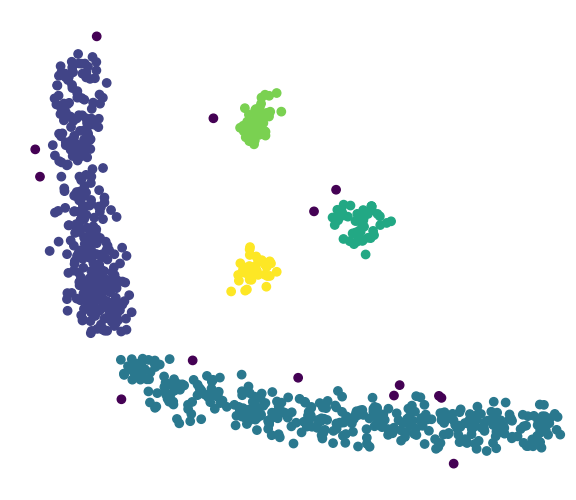
\includegraphics[width=.2\textwidth]{myplot5_1.png}
  %\caption{fig1}
  }
  \quad
  \subfigure[$DBSCAN$]{
  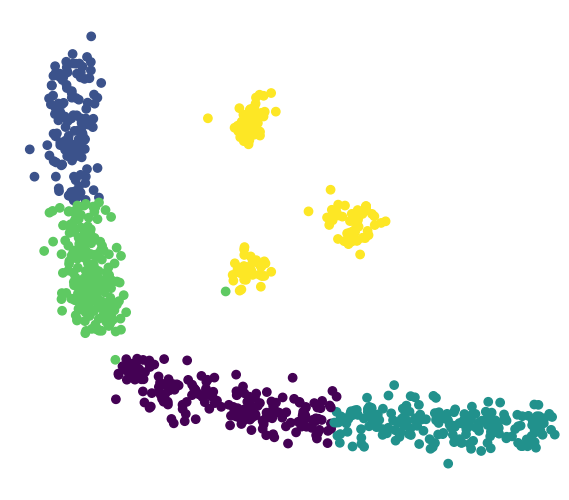
\includegraphics[width=.2\textwidth]{myplot5_2.png}
  }
  \caption{The comparision of $K-means$ and $DBSCAN$}
  \label{fig19}
  \end{figure}
\section{ODG and MC-ODG Algorithms}
%\vspace{-0.2cm}
This section introduces ODG and MC-ODG algorithms.
The methods based on SMOTE are not able to effectively deal with noise points and cluster distribution data.
The noise in the data will lead to overlapping data distributions after oversampling.
Also, the data point generated by SMOTE cannot preserve the original distributions.
MC-CCR randomly generates points in a certain range without retaining the original distributions of a minority points.
Furthermore, this method may generate too many samples of 
minority points near the noise, which will adversely affect the prediction results.
Aiming at the shortcomings of the above methods, 
we propose ODG and MC-ODG to avoid the problems mentioned above.
\subsection{Overview of ODG}
This section gives an overview of ODG. 
% The whole ODG algorithm process can be roughly divided into clustering 
% minority sample points and generating new samples near borderline points, core points and noise points respectively.
First, we use DBSCAN to divide the minority points into core points, 
borderline points and noise points according 
to data distributions. 
Second, We calculate the number of sample points generated near different types of points.
Third, we systnetic new points.
We use gaussian distribution when we systnetic points near borderline points and core points.
In addition, we use SMOTE to systetic points if minority points cannot form effective clusters.
Some of import parameters we used in this section are shown in Table \ref{table15}.
The overall process of ODG is shown is algorithm \ref{alg1}.
\begin{table}[]
  \caption{Parameters of ODG}
  \label{table15}
  \begin{tabular}{ll}
  \hline
  Parameter             & meaning                                                 \\ \hline
  $eps$                 & parameter of DBSCAN                                     \\
  $min\_pts$            & parameter of DBSCAN                                     \\
  $M$                   & majority points                                         \\
  $m$                   & minority points                                         \\
  $N_{oversampling}$    & the number of oversampled points                        \\
  $N_{core}$            & the number of oversampled points near core points       \\
  $N_{borderline}$      & the number of oversampled points near borderline points \\
  $N_{noise}$           & the number of oversampled points near noise points      \\
  $\alpha_{borderline}$ & ratio of generated points near borderline points        \\
  $\alpha_{noise}$      & ratio of generated points near noise points             \\
  $translations$        & the translations of majority points                     \\
  $clusters$            & the clusters of minority points                         \\ 
  $n_{borderline}$      & the number of generation near a single borderline point \\ 
  $n_{core}$            & the number of generation near one cluster               \\ \hline
  \end{tabular}
  \end{table}
  \begin{algorithm}[tbp]
    \caption{ODG} %算法的名字
    \label{alg1}
    \hspace*{0.02in} {\bf Input:}
    %算法的输入, \hspace*{0.02in}用来控制位置,同时利用 \\ 进行换行
     \\$M$ $\leftarrow$ majority points  \\
     $m$ $\leftarrow$ minority points  \\
     $eps$, $min\_pts$\\
    \hspace*{0.02in} {\bf Output:} %算法的结果输出
    Minority points and Majority points
    \begin{algorithmic}[1]
    \State $m_{core}$, $m_{borderline}$, $m_{noise}$, $clusters$=DBSCAN(m,$eps$,$min\_pts$) % \State 后写一般语句
    \State Calculate $N_{noise}$, $N_{borderline}$ and $N_{core}$.
    %\State $cov\_mats$ $\leftarrow$ Calculate the variance of the core points of each cluster,scale according to the number of core points.
    \State $new\_data$ $\leftarrow$ an empty set.
    \State $translations$ $\leftarrow$ a zero matrix, the same shape as $M$.
    \State $generate\_borderline(N_{borderline},m_{boaderline},translations, new\_data)$
    \State $generate\_core(clusters,N_{core},new\_data)$
    \State $generate\_noise(N_{noise},m_{noise},$new\_data$)$
    \State $M$ $\leftarrow$ $M+translations$
    \State $m$ $\leftarrow$ $m$ concatenate with $new\_data$
    \State \Return $M$,$m$
    \end{algorithmic}
    \end{algorithm}

%\vspace{-0.4cm}
\subsection{Binary imbalanced classification}
%\vspace{-0.1cm}
We give the details of ODG algorithm, which is used to solve the binary classification problems.

\textbf{Clustering} We cluster the minority sample points firstly.
An result of K-MEANS and DBSCAN are shown in Fig. \ref{fig19}.
The same color represents the same cluster.
Obviously, the result of DBSCAN is more 
consistent with the data distribution and can easily detect noise points.
After DBSCAN, 
the minority sample points are divided into three types as mentioned.
SMOTE cannot avoid synthetic points on the line between 
two points belong to different clusters.
After dividing multiple clusters, 
we won't generating sample points between clusters to avoid overlapping.


\textbf{Number of generation} After clustering, 
we determine the value of $N_{borderline}$, 
$N_{core}$ and $N_{noise}$. 
% We assume that the number of majority sample points is $N_{maj}$,
% and the number of minority sample points is $N_{min}$, then the number of oversample points 
$N_{oversampling}$ is calculated as Eq. \ref{equation1}.
\begin{equation}
  \label{equation1}
  N_{oversampling}=N_{maj}-N_{min}
\end{equation}

After obtaining the total number of oversampled samples, 
we need to determine the proportion of generated 
in different regions.
%Sample points should not be generated 
The parameter $\alpha_{borderline}$ can be specified as a hyperparameter or can be adaptive determined based on the ratio of borderline points.In general, $\alpha_{borderline}$ is greater than $\frac{N_{borderline}}{N_{min}}$,
because we prefer to generate data near borderline points,
then the classification surface is biased to minority points.
Fig. \ref{fig20}(a) shows the relation with $\alpha_{borderline}$ and $\frac{N_{borderline}}{N_{min}}$.
$\alpha_{borderline}$ is evaluated according to the Eq. \ref{equation15}.
\begin{equation}
  \label{equation15}
  \alpha_{borderline}=(\frac{N_{borderline}}{N_{min}})^{\frac{1}{2}}
\end{equation}

In fact, we can calculate $\alpha_{borderline}$ in a variety of ways. 
We just need to make sure $\alpha_{borderline}$ is greater 
than $\frac{N_{borderline}}{N_{min}}$, in order
to oversample more points near borderline. 
We could also use the function of 1/3 power, or 1/4 power, etc.
We can also specify $\alpha_{borderline}$ by a hyperparameter
if we want to generate more points near borderline points.
\begin{figure}[tb]
  \centering
  \subfigure[$\alpha_{borderline}$]{
  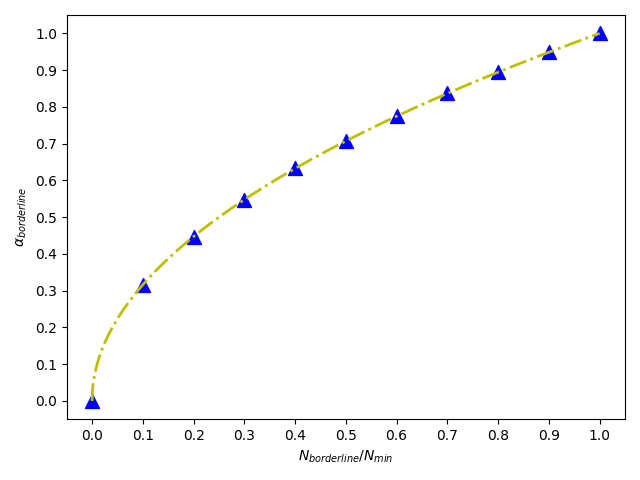
\includegraphics[width=.2\textwidth]{myplot10.png}
  %\caption{fig1}
  }
  \quad
  \subfigure[$\alpha_{noise}$]{
  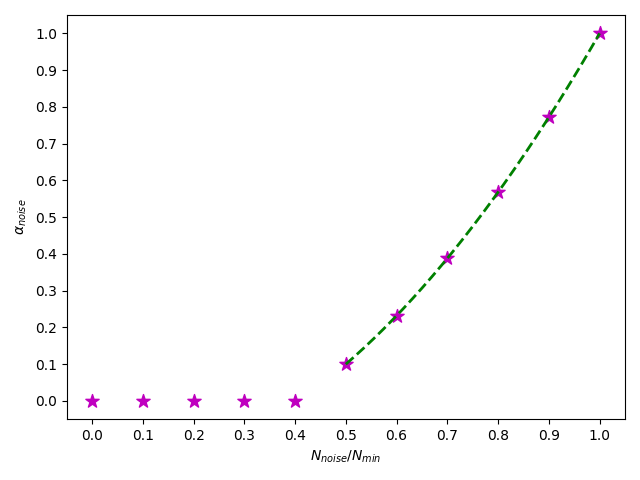
\includegraphics[width=.2\textwidth]{myplot11.png}
  }
  \caption{}
  \label{fig20}
  \end{figure}


In general, 
we separate the noise points by DBSCAN algorithm,
We ignore the noise during oversampling to avoid the impact of noise.
so no new sample points will be synthesized near noise points.
Only when minority points cannot form effective clusters, that is,
most of the sample points are marked as noise points, 
such as when the ratio of noise points $ratio$ exceeds a certain 
super-parameter $noise\_ratio$(generally set as 0.5),
part of new samples will be synthesized near noise points.
As the amount of noise sample point data increases, 
the ratio of generated data near noise points also increases. 
The proportion of samples generated near noise point
 is $\alpha_{noise}$ is shown in Eq. \ref{equation10}.
\begin{equation}
  \label{equation10}
  \alpha_{noise}=
  \begin{cases}
  \frac{0.9}{1-{noise\_{ratio}}^2}\times ratio^2+1-\frac{0.9}{1-{noise\_ratio}^2} & ratio \ge noise\_ratio\\
  0                                                                               & ratio < noise\_ratio
  \end{cases}
\end{equation}

The reason for using Eq. \ref{equation10} is that when $ratio$ is exactly
$noise\_ratio$, the generated ratio is $0.1$. Similar with $borderline\_ratio$,
We can also have many methods to calculate $\alpha_{noise}$,
we use the quadratic function curve similarly with $\alpha\_borderline$ in our work.
When the $noise\_ratio$ is 0.5, the trend of $\alpha_{noise}$ is shown in Fig. \ref{fig20}(b).
We calculate $N_{noise}$ first, and then determine the value of $N_{borderline}$ and $N_{core}$.
$N_{noise}$, $N_{borderline}$ 
and $N_{core}$ are shown in Eq. \ref{equation11}, Eq. \ref{equation16}
and Eq. \ref{equation17}.
\begin{align}
  \label{equation11} & N_{noise}=\alpha_{noise} \times N_{oversampling} \\
  \label{equation16} & N_{borderline}=(N_{oversampling}-N_{noise})\times \alpha_{borderline}\\
  \label{equation17} & N_{core}=N_{oversampling}-N_{borderline}-N_{noise}
\end{align}

\textbf{Generate data near borderline points}
\begin{algorithm}[tb]
  \caption{$generate\_borderline$}
  \label{alg3}
  \hspace*{0.02in} {\bf Input:} %算法的输入, \hspace*{0.02in}用来控制位置,同时利用 \\ 进行换行
   $N_{borderline}$,$m_{borderline}$,$translations$,$new\_data$
  \begin{algorithmic}
    \For{$point$ in $m_{borderline}$} % For 语句,需要和EndFor对应
      \State Calculate K nearest neighbors of $point$.
      \State $cov\_mat$ $\leftarrow$ covariance matrix of the core points related to $point$.
      \State $num\_core\_points$ $\leftarrow$ The number of core points in the same cluster as $point$.
      \State $cov\_mat=cov\_mat/num\_core\_points$
      \State $d\_max$ $\leftarrow$ maximum distance of knearest neighbors.
     \State $n_{borderline}=\frac{n\_knearest\_maj}{\sum_{i\in m} n\_knearest\_maj}\times N_{boardline}$
      \State $tem\_data=multivariate\_normal(point,cov\_mat,n_{borderline})$
      \State add $tem\_data$ to $new\_data$.
      \For{$m_{j}$ in $k\_nearest\_maj$}
        \State $translations_j$=$translations_j$+$\frac{d_{max}-d_{j}}{d_{j}}\times (m_{j}-point)$
      \EndFor
  \EndFor
  \end{algorithmic}
\end{algorithm}
% In order to make the distribution of the generated new sample points 
% consistent with the core
% points corresponding to the borderline point, 
% gaussian distribution is adopted.
We first need to determine $n_{boardline}$ for a particular borderline point.
Then we calculate the K nearest neighbors of each borderline point, 
if the K nearest neighbors of the minority point have more majority sample points, 
means the point 
is closer to the decision boundary, and more sample points should be generated near this point.
We set the number of majority sample points is $n\_knearest\_maj$,
then $n_{boardline}$ can be obtained in Eq. \ref{equation4}.
\begin{equation}
  \label{equation4}
  n_{borderline}=\frac{n\_knearest\_maj}{\sum_{i\in m} n\_knearest\_maj}\times N_{boardline}
\end{equation}

In order to make the distribution of the generated new sample points 
consistent with original data distributions,
gaussian distribution is adopted.
After clustering, each borderline point corresponds to a certain cluster, 
and the core points of this cluster can best represent the cluster's distribution.
Therefore we calculate the covariance matrix of the core points. 
% then use gaussian distribution to generate sample points at the 
% corresponding borderline points after scaling it.
But we cannot use the matrix directly, we 
assume the number of core points in this cluster is $num\_core\_points$,
we need to scale the matrix by $num\_core\_points$ to limit 
the scope of the generated points.
We set the particular borderline point is $point$, 
$cov$ is the function to calculate the covariance matrix,
The function to generate new sample points using 
gaussian distribution is $multivariate\_normal$,
New sample points $new\_data$ can be obtained by Eq. \ref{equation3}.
\begin{equation}
  \label{equation3}
  \begin{aligned}
      & cov\_mat=cov(core\_points)/num\_core\_points \\
      & new\_data=multivariate\_normal(point,cov\_mat,n_{boardline})
  \end{aligned}
\end{equation}
The algorithm for generating new sample points near borderline points is algorithm \ref{alg3}.
%\vspace{-0.4cm}

\textbf{Generate data near core points}
\begin{algorithm}[tb]
  \caption{$generate\_core$}
  \label{alg4}
  \hspace*{0.02in} {\bf Input:} $clusters$,$N_{core}$,$new\_data$
  \begin{algorithmic}
    \For{$cluster$ in $clusters$}
    \State $n_{core}=\frac{num\_data\_cluster}{\sum_{i \in cluster} num\_data\_cluster} \times N_{core}$
    \State $core\_points$ $\leftarrow$ core points of $cluster$
    \State $cov\_mat=cov(core\_points)$
    \State $tem\_data=multivariate\_normal(mean(core\_points),cov\_mat,n_{core})$
    \State add $tem\_data$ to $new\_data$
  \EndFor
  \end{algorithmic}
\end{algorithm}
We generate new data from the mean and variance of the 
core points of each cluster using gaussian distribution.
After DBSCAN, 
the number of generation near the core points of each cluster depends 
on the number of sample points in the cluster.
We assume the number of sample points in the cluster is $num\_data\_cluster$, 
 the number of generalization in this cluster is $n_{core}$, as shown in Eq. \ref{equation6}.
 \begin{equation}
  \label{equation6}
  n_{core}=\frac{num\_data\_cluster}{\sum_{i \in cluster} num\_data\_cluster}
\end{equation}
  
The generation method is similar to that near the borderline points. 
We assume the distribution of sample points in a single cluster obeys gaussian distribution.
The Eq. \ref{equation7} is to generate new sample points near core points.
\begin{equation}
  \label{equation7}
  \begin{aligned}
    & cov\_mat=cov(core\_points) \\
    & new\_data=multivariate\_normal(mean(core\_points),cov\_mat,n_{core})
  \end{aligned}
\end{equation}
The algorithm for generating new sample points at core points is algorithm \ref{alg4}.

%\vspace{-0.4cm}
\textbf{Generate data near noise points}
\begin{algorithm}[tb]
  \caption{$generate\_noise$}
  \label{alg5}
  \hspace*{0.02in} {\bf Input:} $N_{noise}$,$m_{noise}$,$new\_data$
  \begin{algorithmic}
    \For{i from 1 to $N_{noise}$}
    \State point $\leftarrow$ random choice from $m_{noise}$
    \State $new\_point$ $\leftarrow$ using SMOTE to generate a new sample on point
    \State add $new\_point$ to $new\_data$
    \EndFor
  \end{algorithmic}
\end{algorithm}
we use the most basic SMOTE for generation near the noise points.
Gaussian distribution cannot be used for generation because effective clusters cannot be generated. 
Therefore SMOTE is used.
A single sample is randomly selected from the $K$ nearest neighbors of the minority point, 
 and sample points are randomly generated on the line between the two points.
 We set $\gamma \in [0,1]$ is a random value, the two points are $point1$ and $point2$,
 then the generation equation is Eq. \ref{equation9}.
 \begin{equation}
  \label{equation9}
  new\_point=point1+\gamma \times (point2-point1)
\end{equation}

\begin{figure}[tb]
  \centering
  \subfigure[]{
  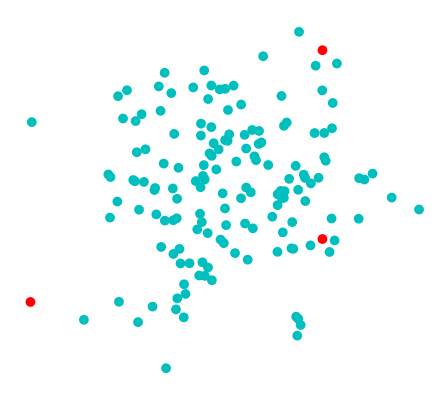
\includegraphics[width=.2\textwidth]{myplot3_1.png}
  %\caption{fig1}
  }
  \quad
  \subfigure[]{
  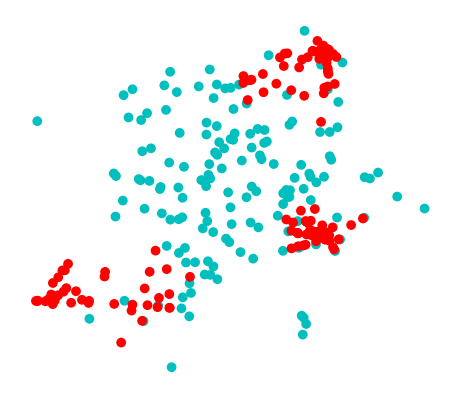
\includegraphics[width=.2\textwidth]{myplot3_2.png}
  }
  \caption{(a) and (b) are distribution of original data and distribution of oversampled data.
  Minority points in the dataset are too rare and far apart to form effective cluster. 
  We use SMOTE to generate new points.}
  \label{fig14}
  \end{figure}

As shown in Fig. \ref{fig14}, (a) and (b) are distribution of original data and 
distribution of oversampled data.
Minority samples in the dataset are too rare and far apart to form effective cluster, we cannot use
gaussian distribution to generate new points, we use SMOTE instead.
Algorithm $generate\_noise$ \ref{alg5} is used to generate new sample points near the noise point.

\textbf{Translation of majority points}
New samples are generated according to the 
distribution characteristics of minority points. 
At the same time we also clean the majority points
 near minority points to alleviate the overlapping data distributions.
We use a similar approach to the model CCR \cite{2017CCR}.
When dealing with borderline points, 
the K nearest neighbors of each minority point is calculated. 
With this minority point as the center and the maximum distance in the K neighbors as the radius, 
a spherical region is drawn. We move the majority points in these K neighbors out of this region.

\begin{figure}[tb]
  \centering
  \subfigure[Original]{
  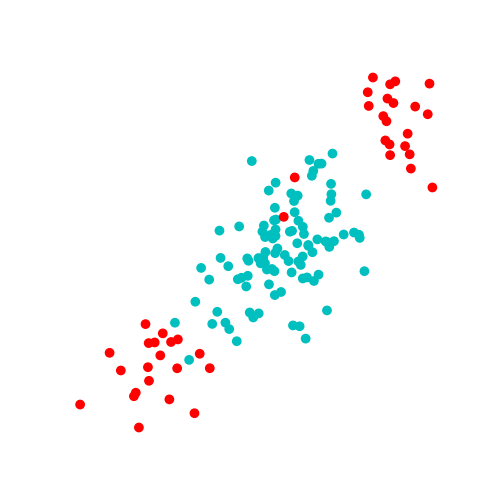
\includegraphics[width=.2\textwidth]{myplot20_0.png}
  %\caption{fig1}
  }
  \quad
  \subfigure[SMOTE]{
  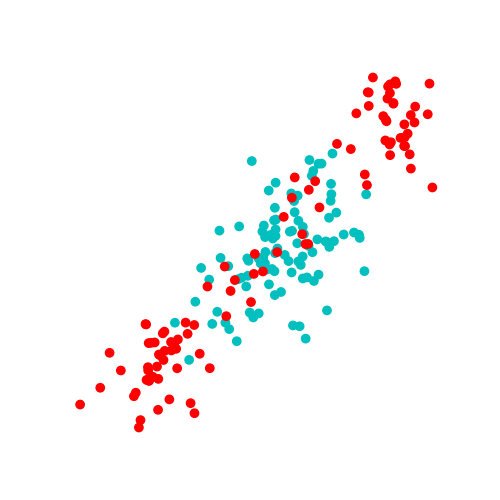
\includegraphics[width=.2\textwidth]{myplot20_1.png}
  }
  \quad
  \subfigure[CCR]{
  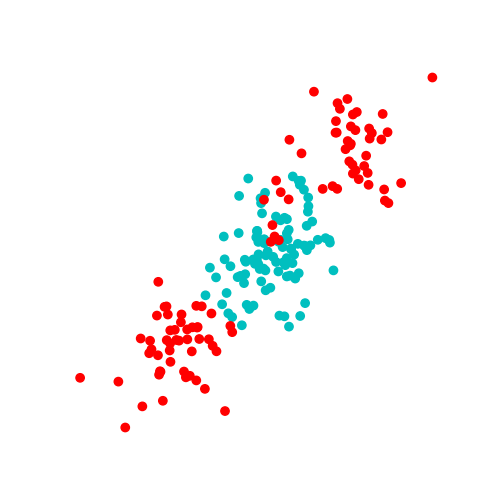
\includegraphics[width=.2\textwidth]{myplot20_2.png}
  }
  \quad
  \subfigure[ODG]{
    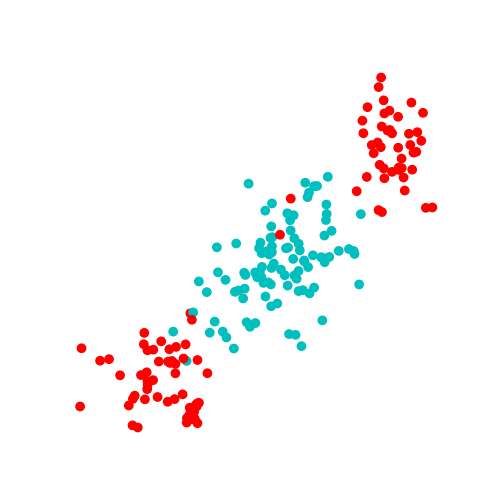
\includegraphics[width=.2\textwidth]{myplot20_3.png}
    }
  \caption{(a) is Original dataset。
  (b),(c),(d) are the oversampling results of SMOTE, CCR and ODG.}
  \label{fig18}
  \end{figure}


We compare the result of SMOTE, CCR and ODG. We assume that some noise points exist in the original data set, 
as well as clustered minority points. The result shows in Fig. \ref{fig18}. 
We can find that after SMOTE, there are overlapping regions, many generated minority points 
overlap with majority points.
Although CCR algorithm avoided overlapping, 
but some minority points were synthesized near the noise, which may produce some interference to predicting results.
\begin{figure}[tb]
  \centering
  \subfigure[Original dataset]{
  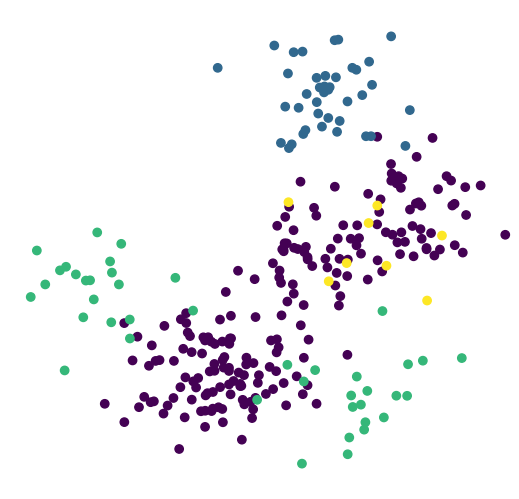
\includegraphics[width=.16\textwidth]{myplot7_1.png}
  %\caption{fig1}
  }
  \quad
  \subfigure[SMOTE]{
  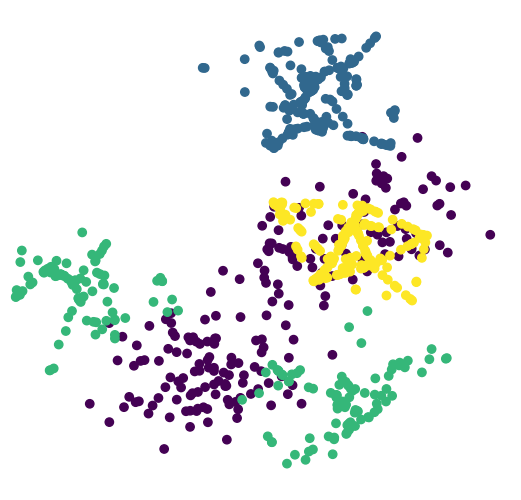
\includegraphics[width=.16\textwidth]{myplot7_2.png}
  }
  \quad
  \subfigure[Borderline-SMOTE]{
  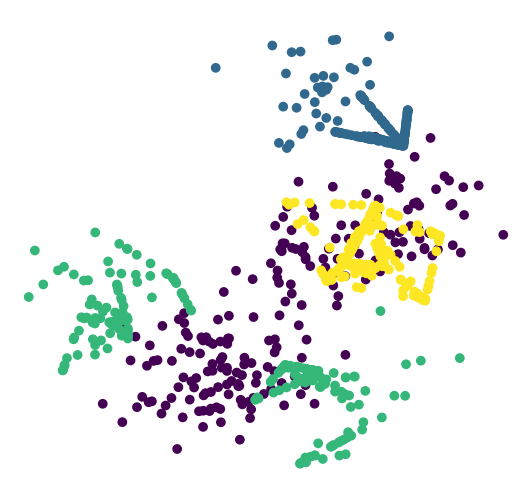
\includegraphics[width=.16\textwidth]{myplot7_3.png}
  }

  \quad
  \subfigure[SMOTE+ENN]{
  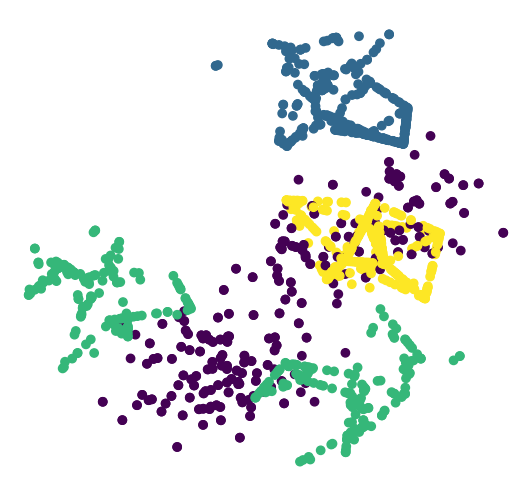
\includegraphics[width=.16\textwidth]{myplot7_4.png}
  }
  \quad
  \subfigure[MC-ODG]{
  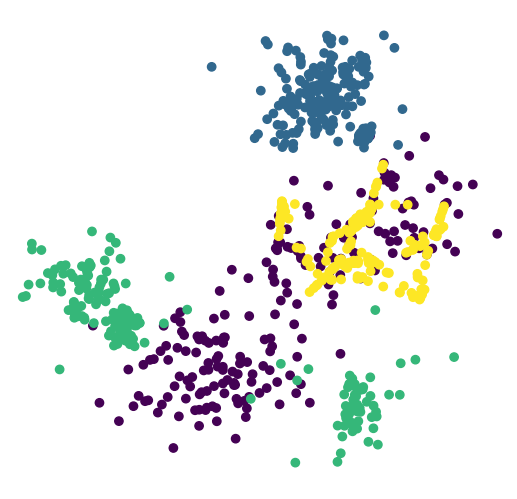
\includegraphics[width=.16\textwidth]{myplot7_5.png}
  }
  \caption{(a) is Original dataset。(b)(c)(d)(e) are oversampling result of SMOTE, 
  Borderline-SMOTE, SMOTE+ENN and MC-ODG.}
  \label{fig17}
  \end{figure}

\textbf{Computational complexity analysis}
We present the time complexity of the oversampling method ODG.
We define the number of majority points is $N_{maj}$, 
the number of minority points is $N_{min}$, the total number of samples is $N$, 
and the number of attributes on the dataset is $m$.
In the DBSCAN algorithm, the time complexity can be controlled at $O(mN_{min}\log(N_{min})$.
which can be simplied to $O(mNlog(N))$.
When calculating the K nearest neighbors of minority points,
The distance between sample points needs to be calculated and sorted, and the complexity of this step is
$O(mN_{min}N+N_{min}Nlog(N))$, it can be simplied as $O(mN^2)$. Therefore the time complexity of
ODG is $O(mN(N+log(N)))$.

%\vspace{-0.4cm}
\subsection{Multiple classification problem}
%\vspace{-0.2cm}

Multiclassification on imbalance dataset is more difficult to solve than that of binary problem. 
\begin{algorithm}[tb]
    \caption{MC-ODG} %算法的名字
    \setlength{\abovedisplayskip}{3pt}
    \setlength{\belowdisplayskip}{3pt}
    \label{alg2}
    \hspace*{0.02in} {\bf Input:} %算法的输入, \hspace*{0.02in}用来控制位置,同时利用 \\ 进行换行
     $X$ $\leftarrow$ a data matrix,which has multiple different labels.  \\
     $C$ $\leftarrow$ different classes
    \hspace*{0.02in} {\bf Output:} %算法的结果输出
     $X$ $\leftarrow$ A new data matrix which has been translated and oversamped.
    \begin{algorithmic}[1]
     
    \For{$i \leftarrow 1$ to $|C|$} % For 语句,需要和EndFor对应
      \State $n_{classes}$ $\leftarrow$ number of classes with higher number of points than $C_i$ 
      \If{$n_{classes}$>0}
          \State $X_{min} \leftarrow X^{C_i}$ 
          \State $X_{maj} \leftarrow \emptyset$
          \For{$j \leftarrow 1$ to $n_{classes}$}
              \State add $\lfloor \frac{|X^{C_1}|}{n_{classes}} \rfloor$ randomly chosen points from $X^{(j)}$ to $X_{maj}$
          \EndFor
          \State $X_{maj}^{'},S=ODG(X_{maj},X_{min})$
          \State $X^{C_i} \leftarrow X^{C_i} \cup S$
          \State substitute points used to construct $X_{maj}$ with $X_{maj}^{'}$. 
        \EndIf
    \EndFor
    \State \Return X
    \end{algorithmic}
    \end{algorithm}

 In the binary classification, 
it is easy to distinguish the majority class and the minority class. 
However, in the multi-classification problem, the relationship between
classes is more complex and difficult to deal.
% It is possible to have multiple majority classes or minority classes.
% A single class can act as a majority towards some classes, a minority towards others.
In addition, overlapping and noise problems will be more serious.
%The existing approaches to multiclassification can be broadly divided into OVA and OVO\cite{articlemulti},
%We assume that there are m classes, and the OVA problem transforms the multiple 
%classification problem into m binary poblems,
%each taking one as a class separately and leaving the remaining classes as another.
%OVO requires training $m(M-1)/2$ binary classifiers, with one classifier trained between two classes.
%There are problems with both methods.
%The OVA method ignores the information between classes that are merged into a unified class,
%With the increase of the number of categories, the complexity of the OVO method increases rapidly.
The traditional OVA and OVO methods have their own disadvantages,  
\cite{2020Combined,2019Radial} presents a method to deal with multiclassification problems,
Combine this method with ODG, we get our algorithm MC-ODG for multiclassification.
We iterate over multiple classes. When we oversample each class,
A subset is selected as a majority class from the already processed classes, 
and this class is treated as a minority class.
We first sort the classes in reverse order according to the number of samples, and for each minority class, 
from the ones that have been processed,
select a subset of the majority classes, and mark the minority class as the majority class 
after processing the ODG algorithm.
Start from the second largerst class, each class can be treated as minority class.
Each majority class has the same number of samples during sampling.
This algorithm makes use of the distribution of 
other majority points when oversampling each class.
The overall process of the MC-ODG algorithm is shown in the algorithm \ref{alg2}.


 Fig. \ref{fig17} shows the original dataset and the oversampling results of SMOTE, Borderline-SMOTE,
 SMOTE+ENN and MC-ODG. We can find that the original data distributions 
 can be retained after oversampling using the $MC-ODG$ algorithm.

%\vspace{-0.4cm}
 \textbf{Computational complexity analysis}
We calculate the time complexity of MC-ODG.
 We also define the total number of samples is N, and the number of attributes on the dataset is $m$.
 The number of classes is $c$. The entire MC-ODG process is equivalent to c-1 times ODG.
 Therefore the time complexity of MC-ODG is $O(cmN(N+log(N)))$.

 %\vspace{-0.4cm}
\section{Experiments}
%\vspace{-0.2cm}

In this section, we will detail a series of experiments on ODG and MC-ODG.
We compared the ODG, MC-ODG algorithms with the existing oversampling methods,
We published the code of our model on github\footnote{https://github.com/Xiaoctw/MC-ODG}.
We ran our code on Intel(R) Xeon(R) CPU E5-2678.
%\vspace{-0.4cm}
\subsection{Evaluation matrics}
%\vspace{-0.1cm}

We evaluated different oversampling algorithms using different metrics. 
Prediction accuracy is not a good metric on imbalanced problems.
Due to the imbalance of data, the accuracy will naturally incline to the majority class.
The predictive ability of the model for minority classes cannot be reflected by accuracy.
%\vspace{-0.4cm}

\textbf{Binary classification} We labeled the majority class as 0(Negative) and the minority class as 1(Positive).
Precision, Recall, F-value and Auc are more reasonable metrics.
Table \ref{table1} gives the confusion matrix for the binary classification problems.
Using the confusion matrix, 
  we can calculate the Precision, Recall and F-value. The calculation formulas are as follows:

\begin{table}[tb]
  \caption{Confusion matrix for the two-class problem}
  \label{table1}
  \centering
  \begin{tabular}{@{}ccc@{}}
  \toprule
  Actual label & \multicolumn{1}{l}{Predicted positive} & \multicolumn{1}{l}{Predicted negative} \\ \midrule
  Positive     & TP                                     & FP                                     \\
  Negative     & FP                                     & FN                                     \\ \bottomrule
  \end{tabular}
\end{table}

  \begin{equation}
    \begin{aligned}
    & Precision=\frac{TP}{TP+FP}  \\ 
    & Recall=\frac{TP}{TP+FN}     \\
    & F-value=\frac{(1+\beta^2) \times Precision \times Recall}{\beta^2 \times Precision+Recall}
  \end{aligned}
  \end{equation}
  The value of Auc is defined as the area bounded by the curve of $roc$ and the coordinate axis.
In general, the value of Auc is greater than 0.5. 
The closer the value is to 1, the better the prediction result is.
%\vspace{-0.4cm}

\textbf{Multiple classification}
The evaluation of multiclassification is more complex,
 and there is not a unified evaluation standard and it is still an open problem.
 In addition to the above mentioned Precision, Recall and F-value,
 mGM and CBA \cite{2017Relevance} are also introduced.
 The equation of CBA and mGM are as follow:
\begin{align}
    \label{equation13}  & mGM=\sqrt[M]{\Pi_{i=1}^M Recall_{i}} \\
    \label{equation12}  & CBA=\frac{\sum_{i=1}^{M}\frac{mat_{i,j}}{max(\sum_{j=1}^Mmat_{i,j},\sum_{j=1}^M mat_{j,i})}}{M}
\end{align}
%\vspace{-0.4cm}

\subsection{Dataset}
%\vspace{-0.1cm}
\begin{table}[tb]
    \caption{Binary and multiple classification datasets}
    \label{table14}
    \begin{tabular}{cccccc}
    \hline
    Datasets        & Instances & Features & Classes & Class distribution               & IR    \\ \hline
    Transfusion(TR) & 748       & 5        & 2       & 570/178                          & 3.2   \\
    Wisconsin(WIS)  & 699       & 25       & 2       & 458/241                          & 1.9   \\
    Adult(AD)       & 32561     & 108      & 2       & 24720/7841                       & 3.2   \\
    Haberman(HA)    & 336       & 3        & 2       & 225/81                           & 2.8   \\
    Glass(GL)       & 213       & 8        & 6       & 76/69/29/17/13/9                 & 8.4   \\
    Automobile(AU)  & 159       & 25       & 6       & 48/46/29/13/3                    & 16    \\
    Wine(WI)        & 157       & 12       & 3       & 71/58/48                         & 1.5   \\
    Yeast(YE)       & 1484      & 7        & 10      & 463/429/244/163/51/44/35/30/20/4 & 115.6 \\
    Ecoli(EC)       & 336       & 6        & 8       & 143/77/52/35/20/5/2/2            & 71    \\ \hline
    \end{tabular}
    \end{table}

The dataset used in the experiment is the classification 
datasets on UCI\footnote{http://archive.ics.uci.edu/ml/datasets.php},
datasets' details are in table %table\ref{table3} and table\ref{table2}.
\ref{table14}.
%\vspace{-0.4cm}

\subsection{Experiment results and analysis}
%\vspace{-0.1cm}

We compared the prediction results of different oversampling models.
In this experiment, we used three widely used machine learning models, C4.5, KNN and LR.
We compared different oversampling methods, SMOTE, Borderline-SMOTE, ADASYN, SMOTE+ENN, MC-CCR 
and ODG or MC-ODG.
we adopted the cross validation method of K folding, 
set K=5, repeated the experiment for 10 times, 
and took the mean value as the final result.
Parameters of ODG, MC-ODG and other algorithms are shown in table \ref{table13}.
$fit\_borderline\_ratio$ means being 
adaptive to determine the $borderline\_ratio$ or not.
We gave a comparison of different oversampling methods on different 
datasets based using different machine learning models.  
The parameters of DBSCAN n are $eps$ and $min\_pts$.
$borderline\_ratio$ of some datasets is artificially specified.
Parameter settings on different datasets are shown in table \ref{table5}.
When the parameter had multiple optional values, we took the optimal result.
\begin{table}[tb]
  \caption{Parameters of different algorithms}
  \label{table13}
  \centering
  \begin{tabular}{cccc}
  \hline
  Algorithm        & Parameters                                                                                                                                                                                              & Algorithm                                             & Parameters                                                                                                                                                   \\ \hline
  MC-CCR           & \multicolumn{1}{c|}{\begin{tabular}[c]{@{}c@{}}$energy \in [0.25,0.5,1]$\\ cleaning strategy: translation\\ selection strategy: proportional\\ multi-class decomposition method: sampling\end{tabular}} & \begin{tabular}[c]{@{}c@{}}ODG\\ /MC-ODG\end{tabular} & \begin{tabular}[c]{@{}c@{}}k=5\\ eps=0.08\\ min\_pts=4\\ fit\_borderline\_ratio=true\\ borderline\_ratio=0.6\\ noise\_ratio=0.1\end{tabular}                 \\ \hline
  SMOTE            & \multicolumn{1}{c|}{k\_neighbors $\in [3,5,7]$}                                                                                                                                                         & KNN                                                   & k $\in [3,5,7]$                                                                                                                                              \\ \hline
  Borderline-SMOTE & \multicolumn{1}{c|}{\begin{tabular}[c]{@{}c@{}}k\_neighbors $\in [3,5,7]$\\ kind="borderline-1"\end{tabular}}                                                                                           & C4.5                                                  & \begin{tabular}[c]{@{}c@{}}max\_depth=5\\ min\_samples\_splits=3\end{tabular}                                                                                \\ \cline{1-2}
  ADASYN           & \multicolumn{1}{c|}{n\_neighbors $\in [3,5,7]$}                                                                                                                                                         &                                                       &                                                                                                                                                              \\ \cline{1-2}
  SMOTE+ENN        & \multicolumn{1}{c|}{k\_neighbors $\in [3,5,7]$}                                                                                                                                                         &                                                       &                                                                                                                                                              \\ \hline
  \end{tabular}
  \end{table}
  \begin{table}[]
    \caption{Parameters of ODG, MC-ODG}
  \label{table5}
   \centering
    \begin{tabular}{cc|cc}
    \hline
    \multicolumn{1}{c|}{Datasets} & Parameters                                                                            & \multicolumn{1}{c|}{Datasets} & Parameters                                                                                    \\ \hline
    TR                            & \begin{tabular}[c]{@{}c@{}}eps=0.15\\ min\_pts=3\\ borderline\_ratio=0.5\end{tabular} & GL                            & \begin{tabular}[c]{@{}c@{}}eps=0.15\\ min\_pts=3\end{tabular}                                 \\ \hline
    WIS                           & \begin{tabular}[c]{@{}c@{}}eps=0.5\\ min\_pts=3\\ borderline\_ratio=0.7\end{tabular}  & AU                            & \begin{tabular}[c]{@{}c@{}}eps=1.8\\min\_pts=3\\ borderline\_ratio=0.4\\ noise\_ratio=0.2\end{tabular} \\ \hline
    AD                            & \begin{tabular}[c]{@{}c@{}}eps=1.6\\ min\_pts=5\\ borderline=0.7\end{tabular}         & WI                            & \begin{tabular}[c]{@{}c@{}}eps=0.36\\ min\_pts=2\end{tabular}                                 \\ \hline
    HA                            & \begin{tabular}[c]{@{}c@{}}eps=0.14\\ min\_pts=3\end{tabular}                         & EC                            & \begin{tabular}[c]{@{}c@{}}eps=0.14\\min\_pts=3\end{tabular}                    \\ \hline
                                  &                                                                                       & YE                            & \begin{tabular}[c]{@{}c@{}}eps=0.13\\min\_pts=3\end{tabular} \\ \hline
    \end{tabular}
    \end{table}
For binary datasets, KNN, C4.5 and LR results on multiple metrics are shown 
in table \ref{table7}, table \ref{table8} and table \ref{table9}. 
For multiclassification datasets, KNN, C4.5 and LR 
results in table \ref{table10} and table \ref{table11} and table \ref{table12}.
\begin{table}[]
  \caption{KNN model deals with binary classification datasets}
  \setlength{\abovedisplayskip}{3pt}
  \setlength{\belowdisplayskip}{3pt}
  \label{table7}
  \resizebox{\textwidth}{15mm}{
    \begin{tabular}{@{}ccccccccccccccccc@{}}
      \toprule
      \multicolumn{1}{c|}{\multirow{2}{*}{Datasets}}  & \multicolumn{4}{c|}{Precision}                                                                                                               & \multicolumn{4}{c}{Recall}                                                                                                                   & \multicolumn{4}{c|}{F1-score}                                                                                                                & \multicolumn{4}{c}{Auc}                                                                                                               \\ \cmidrule(l){2-17} 
      \multicolumn{1}{c|}{}                           & \multicolumn{1}{c|}{TR}          & \multicolumn{1}{c|}{WIS}                     & \multicolumn{1}{c|}{AD}    & \multicolumn{1}{c|}{HA}       & \multicolumn{1}{c|}{TR}          & \multicolumn{1}{c|}{WIS}                     & \multicolumn{1}{c|}{AD}    & \multicolumn{1}{c|}{HA}       & \multicolumn{1}{c|}{TR}          & \multicolumn{1}{c|}{WIS}                     & \multicolumn{1}{c|}{AD}    & \multicolumn{1}{c|}{HA}       & \multicolumn{1}{c|}{TR}          & \multicolumn{1}{c|}{WIS}                     & \multicolumn{1}{c|}{AD}    & \multicolumn{1}{c}{HA}        \\ \midrule
      Original dataset                                & 0.823                            & 0.934                                        & 0.823                      & 0.426                         & 0.646                            & 0.921                                        & 0.839                      & 0.282                         & 0.717                            & 0.926                                        & 0.83                       & 0.332                         & 0.837                            & 0.955                                        & 0.913                      & 0.604                         \\
      SMOTE                                           & 0.843                            & 0.926                                        & 0.819                      & 0.465                         & 0.604                            & 0.935                                        & 0.837                      & 0.337                         & 0.7                              & 0.93                                         & 0.827                      & 0.381                         & 0.824                            & 0.954                                        & 0.912                      & 0.617                         \\
      Borderline-SMOTE                                & 0.853                            & 0.93                                         & 0.824                      & 0.421                         & 0.606                            & 0.91                                         & 0.839                      & 0.269                         & 0.706                            & 0.919                                        & 0.83                       & 0.319                         & 0.827                            & 0.949                                        & 0.912                      & 0.621                         \\
      ADASYN                                          & \textbf{0.873}                   & \textbf{0.937}                               & 0.819                      & \textbf{0.452}                & 0.618                            & 0.912                                        & 0.843                      & 0.36                          & \textbf{0.721}                   & 0.924                                        & 0.829                      & 0.383                         & 0.834                            & 0.95                                         & 0.913                      & 0.619                         \\
      SMOTE+ENN                                       & 0.71                             & 0.921                                        & 0.797                      & 0.412                         & 0.677                            & 0.953                                        & 0.876                      & 0.537                         & 0.69                             & 0.936                                        & 0.831                      & 0.46                          & 0.806                            & 0.958                                        & 0.912                      & 0.64                          \\
      CCR                                             & 0.738                            & 0.925                                        & 0.794                      & 0.368                         & \textbf{0.808}                   & 0.94                                         & 0.862                      & \textbf{0.626}                & 0.709                            & 0.931                                        & 0.825                      & 0.457                         & 0.834                            & 0.958                                        & 0.909                      & 0.622                         \\
      ODG                                             & 0.8                              & 0.921                                        & \textbf{0.831}             & \textbf{0.452}                & 0.75                             & \textbf{0.956}                               & \textbf{0.879}             & 0.517                         & 0.711                            & \textbf{0.938}                               & \textbf{0.84}              & \textbf{0.476}                & \textbf{0.846}                   & \textbf{0.965}                               & \textbf{0.916}             & \textbf{0.667}                \\ \bottomrule
      \end{tabular}
  }
  \end{table}
\begin{table}[]
    \caption{C4.5 model deals with binary classification datasets}
    \label{table8}
    \setlength{\abovedisplayskip}{3pt}
    \setlength{\belowdisplayskip}{3pt}
    \resizebox{\textwidth}{15mm}{
      \begin{tabular}{@{}ccccccccccccccccc@{}}
        \toprule
        \multicolumn{1}{c|}{\multirow{2}{*}{Datasets}}  & \multicolumn{4}{c|}{Precision}                                                                                                               & \multicolumn{4}{c}{Recall}                                                                                                                   & \multicolumn{4}{c|}{F1-score}                                                                                                                & \multicolumn{4}{c}{Auc}                                                                                                               \\ \cmidrule(l){2-17} 
        \multicolumn{1}{c|}{}                           & \multicolumn{1}{c|}{TR}          & \multicolumn{1}{c|}{WIS}                     & \multicolumn{1}{c|}{AD}    & \multicolumn{1}{c|}{HA}       & \multicolumn{1}{c|}{TR}          & \multicolumn{1}{c|}{WIS}                     & \multicolumn{1}{c|}{AD}    & \multicolumn{1}{c|}{HA}       & \multicolumn{1}{c|}{TR}          & \multicolumn{1}{c|}{WIS}                     & \multicolumn{1}{c|}{AD}    & \multicolumn{1}{c|}{HA}       & \multicolumn{1}{c|}{TR}          & \multicolumn{1}{c|}{WIS}                     & \multicolumn{1}{c|}{AD}    & \multicolumn{1}{c}{HA}        \\ \midrule
        Original dataset                                & 0.841                            & 0.936                                        & 0.819                      & 0.419                         & 0.6                              & 0.918                                        & 0.848                      & 0.305                         & 0.697                            & 0.926                                        & 0.832                      & 0.34                          & 0.823                            & 0.959                                        & 0.926                      & 0.623                         \\
        SMOTE                                           & \textbf{0.844}                   & 0.93                                         & 0.823                      & 0.448                         & 0.625                            & 0.923                                        & 0.845                      & 0.316                         & \textbf{0.714}                   & 0.935                                        & 0.832                      & 0.359                         & 0.835                            & 0.957                                        & 0.923                      & 0.605                         \\
        Borderline-SMOTE                                & 0.839                            & 0.931                                        & 0.812                      & \textbf{0.482}                & 0.587                            & 0.922                                        & 0.852                      & 0.315                         & 0.684                            & 0.925                                        & 0.83                       & 0.373                         & 0.816                            & 0.958                                        & 0.924                      & 0.594                         \\
        ADASYN                                          & 0.843                            & 0.928                                        & 0.815                      & 0.475                         & 0.596                            & 0.924                                        & 0.848                      & 0.338                         & 0.694                            & 0.924                                        & 0.83                       & 0.388                         & 0.822                            & 0.957                                        & 0.924                      & 0.627                         \\
        SMOTE+ENN                                       & 0.697                            & 0.919                                        & 0.789                      & 0.41                          & 0.673                            & 0.954                                        & \textbf{0.882}             & 0.552                         & 0.678                            & 0.936                                        & 0.834                      & 0.449                         & 0.799                            & 0.959                                        & 0.927                      & 0.628                         \\
        CCR                                             & 0.751                            & 0.918                                        & 0.79                       & 0.367                         & \textbf{0.809}                   & \textbf{0.954}                               & 0.88                       & \textbf{0.628}                & 0.688                            & 0.935                                        & 0.832                      & \textbf{0.465}                & 0.836                            & 0.965                                        & 0.924                      & 0.635                         \\
        ODG                                             & 0.755                            & \textbf{0.938}                               & \textbf{0.824}             & 0.429                         & 0.681                            & 0.951                                        & 0.859                      & 0.524                         & 0.672                            & \textbf{0.943}                               & \textbf{0.84}              & 0.455                         & \textbf{0.843}                   & \textbf{0.968}                               & \textbf{0.928}             & \textbf{0.656}                \\ \bottomrule
        \end{tabular}
        }   
\end{table}
\begin{table}[]
      \caption{LR model deals with binary classification datasets}
      \label{table9}
      \setlength{\abovedisplayskip}{3pt}
    \setlength{\belowdisplayskip}{3pt}
      \resizebox{\textwidth}{15mm}{
        \begin{tabular}{@{}ccccccccccccccccc@{}}
          \hline
          \multicolumn{1}{c|}{\multirow{2}{*}{Datasets}}  & \multicolumn{4}{c|}{Precision}                                                                                                               & \multicolumn{4}{c|}{Recall}                                                                                                                  & \multicolumn{4}{c|}{F1-score}                                                                                                                & \multicolumn{4}{c}{Auc}                                                                                                              \\ \cmidrule(l){2-17} 
          \multicolumn{1}{c|}{}                           & \multicolumn{1}{c|}{TR}          & \multicolumn{1}{c|}{WIS}                     & \multicolumn{1}{c|}{AD}    & \multicolumn{1}{c|}{HA}       & \multicolumn{1}{c|}{TR}          & \multicolumn{1}{c|}{WIS}                     & \multicolumn{1}{c|}{AD}    & \multicolumn{1}{c|}{HA}       & \multicolumn{1}{c|}{TR}          & \multicolumn{1}{c|}{WIS}                     & \multicolumn{1}{c|}{AD}    & \multicolumn{1}{c|}{HA}       & \multicolumn{1}{c|}{TR}          & \multicolumn{1}{c|}{WIS}                     & \multicolumn{1}{c|}{AD}    & \multicolumn{1}{c}{HA}        \\ \midrule
          Original dataset                                & 0.872                            & \textbf{0.962}                               & 0.848                      & \textbf{0.691}                & 0.571                            & 0.946                                        & 0.84                       & 0.284                         & 0.568                            & 0.953                                        & 0.832                      & 0.261                         & 0.847                            & \textbf{0.996}                               & 0.952                      & 0.663                         \\
          SMOTE                                           & 0.892                            & \textbf{0.962}                               & 0.843                      & 0.673                         & 0.549                            & 0.941                                        & 0.82                       & 0.322                         & 0.536                            & 0.951                                        & 0.829                      & 0.309                         & 0.848                            & 0.995                                        & 0.96                       & 0.642                         \\
          Borderline-SMOTE                                & 0.871                            & 0.961                                        & \textbf{0.857}             & 0.653                         & 0.553                            & 0.946                                        & 0.824                      & 0.286                         & 0.549                            & 0.953                                        & 0.837                      & 0.313                         & 0.845                            & 0.992                                        & 0.961                      & 0.663                         \\
          ADASYN                                          & \textbf{0.921}                   & 0.958                                        & 0.852                      & 0.658                         & 0.553                            & 0.95                                         & 0.828                      & 0.321                         & 0.646                            & 0.953                                        & \textbf{0.839}             & 0.309                         & 0.847                            & 0.995                                        & 0.96                       & 0.644                         \\
          SMOTE+ENN                                       & 0.779                            & 0.951                                        & 0.775                      & 0.536                         & 0.701                            & 0.962                                        & 0.895                      & \textbf{0.569}                & 0.663                            & 0.956                                        & \textbf{0.839}             & 0.443                         & 0.847                            & \textbf{0.996}                               & 0.957                      & 0.658                         \\
          CCR                                             & 0.69                             & 0.951                                        & 0.779                      & 0.525                         & 0.763                            & 0.967                                        & 0.884                      & 0.445                         & \textbf{0.665}                   & 0.958                                        & 0.832                      & 0.396                         & 0.848                            & 0.965                                        & 0.957                      & 0.635                         \\
          ODG                                             & 0.655                            & 0.956                                        & 0.775                      & 0.543                         & \textbf{0.781}                   & \textbf{0.968}                               & \textbf{0.906}             & 0.457                         & 0.657                            & \textbf{0.959}                               & 0.834                      & \textbf{0.457}                & \textbf{0.853}                   & \textbf{0.996}                               & \textbf{0.959}             & \textbf{0.668}                \\ \bottomrule
          \end{tabular}
          } 
\end{table}
\begin{table}[]
        \caption{KNN model deals with multiclassification datasets}
        \label{table10}
        \setlength{\abovedisplayskip}{3pt}
          \setlength{\belowdisplayskip}{3pt}
        \resizebox{\textwidth}{15mm}{
        \begin{tabular}{cccccccccccccccccccccccccc}
        \hline
        \multicolumn{1}{c|}{\multirow{2}{*}{Datasets}}  & \multicolumn{5}{c|}{Precision}                                                                                                                     & \multicolumn{5}{c|}{Recall}                                                                                                                        & \multicolumn{5}{c|}{F1-score}                                                                                                                      & \multicolumn{5}{c|}{mGM}                                                                                                                           & \multicolumn{5}{c}{CBA}                                                                                                                           \\ \cline{2-26} 
        \multicolumn{1}{c|}{}                           & \multicolumn{1}{c|}{AU}         & \multicolumn{1}{c|}{EC}    & \multicolumn{1}{c|}{GL}    & \multicolumn{1}{c|}{WI}   & \multicolumn{1}{c|}{YE}    & \multicolumn{1}{c|}{AU}         & \multicolumn{1}{c|}{EC}    & \multicolumn{1}{c|}{GL}    & \multicolumn{1}{c|}{WI}   & \multicolumn{1}{c|}{YE}    & \multicolumn{1}{c|}{AU}         & \multicolumn{1}{c|}{EC}    & \multicolumn{1}{c|}{GL}    & \multicolumn{1}{c|}{WI}   & \multicolumn{1}{c|}{YE}    & \multicolumn{1}{c|}{AU}         & \multicolumn{1}{c|}{EC}    & \multicolumn{1}{c|}{GL}    & \multicolumn{1}{c|}{WI}   & \multicolumn{1}{c|}{YE}    & \multicolumn{1}{c|}{AU}         & \multicolumn{1}{c|}{EC}    & \multicolumn{1}{c|}{GL}    & \multicolumn{1}{c|}{WI}   & \multicolumn{1}{c}{YE}     \\ \hline
        Original dataset                                & \textbf{0.765}                  & 0.84                       & 0.57                       & 0.962                     & 0.5                        & 0.718                           & 0.78                       & 0.575                      & 0.96                      & 0.492                      & 0.716                           & 0.767                      & 0.555                      & 0.954                     & 0.465                      & 0.713                           & 0.761                      & 0.651                      & 0.958                     & 0.467                      & 0.643                           & 0.717                      & 0.497                      & 0.92                      & 0.419                      \\
        SMOTE                                           & 0.742                           & 0.839                      & 0.572                      & 0.962                     & 0.506                      & 0.695                           & 0.793                      & 0.554                      & 0.969                     & 0.496                      & 0.692                           & 0.802                      & 0.541                      & \textbf{0.963}            & \textbf{0.492}             & 0.643                           & 0.762                      & 0.593                      & \textbf{0.968}            & 0.484                      & 0.618                           & 0.748                      & 0.484                      & 0.931                     & 0.45                       \\
        Borderline-SMOTE                                & 0.716                           & \textbf{0.843}             & 0.578                      & 0.957                     & 0.498                      & 0.677                           & 0.789                      & 0.562                      & 0.963                     & 0.491                      & 0.667                           & 0.802                      & 0.547                      & 0.957                     & 0.486                      & 0.599                           & 0.736                      & 0.633                      & 0.961                     & 0.483                      & 0.591                           & 0.741                      & 0.486                      & 0.924                     & 0.444                      \\
        ADASYN                                          & 0.716                           & \textbf{0.843}             & 0.576                      & 0.955                     & 0.496                      & 0.668                           & 0.793                      & 0.562                      & 0.961                     & 0.494                      & 0.661                           & 0.807                      & 0.547                      & 0.955                     & 0.489                      & 0.621                           & 0.768                      & 0.632                      & 0.959                     & 0.488                      & 0.583                           & 0.756                      & 0.488                      & 0.922                     & 0.449                      \\
        SMOTE+ENN                                       & 0.588                           & 0.823                      & 0.391                      & 0.947                     & \textbf{0.51}              & 0.563                           & 0.815                      & 0.466                      & 0.956                     & 0.485                      & 0.538                           & 0.81                       & 0.401                      & 0.947                     & 0.466                      & 0.481                           & 0.8                        & 0.562                      & 0.953                     & 0.465                      & 0.473                           & \textbf{0.757}             & 0.349                      & 0.903                     & 0.41                       \\
        MC-CCR                                          & 0.719                           & 0.774                      & 0.603                      & 0.955                     & 0.455                      & 0.737                           & 0.803                      & 0.642                      & 0.967                     & 0.5                        & 0.706                           & \textbf{0.811}             & 0.597                      & \textbf{0.963}            & 0.482                      & 0.713                           & 0.775                      & 0.652                      & 0.958                     & \textbf{0.496}             & 0.626                           & 0.717                      & 0.525                      & 0.934                     & 0.445                      \\
        MC-ODG                                          & 0.738                           & 0.805                      & \textbf{0.637}             & \textbf{0.963}            & 0.481                      & \textbf{0.75}                   & \textbf{0.815}             & \textbf{0.664}             & \textbf{0.97}             & \textbf{0.511}             & \textbf{0.721}                  & 0.805                      & \textbf{0.622}             & \textbf{0.963}            & 0.489                      & \textbf{0.725}                  & \textbf{0.803}             & \textbf{0.658}             & 0.967                     & 0.484                      & \textbf{0.641}                  & 0.745                      & \textbf{0.546}             & \textbf{0.935}            & \textbf{0.453}             \\ \hline
        \end{tabular}
        }
\end{table} 
\begin{table}[]
    \caption{C4.5 model deals with multiclassification datasets}
    \label{table11}
    \setlength{\abovedisplayskip}{3pt}
    \setlength{\belowdisplayskip}{3pt}
    \resizebox{\textwidth}{15mm}{
    \begin{tabular}{cccccccccccccccccccccccccc}
    \hline
    \multicolumn{1}{c|}{\multirow{2}{*}{Datasets}}  & \multicolumn{5}{c|}{Precision}                                                                                                                     & \multicolumn{5}{c|}{Recall}                                                                                                                        & \multicolumn{5}{c|}{F1-score}                                                                                                                      & \multicolumn{5}{c|}{mGM}                                                                                                                           & \multicolumn{5}{c}{CBA}                                                                                                                           \\ \cline{2-26} 
    \multicolumn{1}{c|}{}                           & \multicolumn{1}{c|}{AU}         & \multicolumn{1}{c|}{EC}    & \multicolumn{1}{c|}{GL}    & \multicolumn{1}{c|}{WI}   & \multicolumn{1}{c|}{YE}    & \multicolumn{1}{c|}{AU}         & \multicolumn{1}{c|}{EC}    & \multicolumn{1}{c|}{GL}    & \multicolumn{1}{c|}{WI}   & \multicolumn{1}{c|}{YE}    & \multicolumn{1}{c|}{AU}         & \multicolumn{1}{c|}{EC}    & \multicolumn{1}{c|}{GL}    & \multicolumn{1}{c|}{WI}   & \multicolumn{1}{c|}{YE}    & \multicolumn{1}{c|}{AU}         & \multicolumn{1}{c|}{EC}    & \multicolumn{1}{c|}{GL}    & \multicolumn{1}{c|}{WI}   & \multicolumn{1}{c|}{YE}    & \multicolumn{1}{c|}{AU}         & \multicolumn{1}{c|}{EC}    & \multicolumn{1}{c|}{GL}    & \multicolumn{1}{c|}{WI}   & \multicolumn{1}{c}{YE}     \\ \hline
    Original dataset                                & 0.738                           & 0.762                      & 0.658                      & 0.911                     & \textbf{0.541}             & 0.7                             & 0.736                      & 0.63                       & 0.906                     & 0.478                      & 0.695                           & 0.731                      & 0.625                      & 0.904                     & 0.479                      & 0.7                             & 0.723                      & 0.59                       & 0.901                     & 0.574                      & 0.626                           & 0.68                       & 0.567                      & 0.859                     & 0.434                      \\
    SMOTE                                           & 0.702                           & 0.8                        & 0.662                      & 0.934                     & \textbf{0.541}             & 0.685                           & 0.761                      & 0.617                      & 0.918                     & 0.499                      & 0.675                           & 0.768                      & 0.617                      & 0.916                     & 0.5                        & 0.686                           & 0.731                      & 0.639                      & 0.915                     & 0.583                      & 0.614                           & 0.715                      & 0.558                      & 0.873                     & 0.387                      \\
    Borderline-SMOTE                                & 0.741                           & \textbf{0.802}             & 0.67                       & 0.915                     & 0.532                      & 0.718                           & 0.75                       & 0.631                      & 0.908                     & 0.497                      & 0.709                           & 0.759                      & 0.622                      & 0.908                     & 0.498                      & 0.679                           & 0.728                      & 0.594                      & 0.905                     & 0.57                       & 0.642                           & 0.701                      & 0.552                      & 0.869                     & 0.439                      \\
    ADASYN                                          & 0.749                           & 0.789                      & 0.646                      & 0.915                     & 0.539                      & 0.716                           & 0.748                      & 0.619                      & 0.915                     & 0.501                      & 0.708                           & 0.755                      & 0.611                      & 0.912                     & 0.504                      & 0.695                           & 0.739                      & 0.619                      & 0.912                     & 0.576                      & 0.637                           & 0.695                      & 0.543                      & 0.881                     & 0.449                      \\
    SMOTE+ENN                                       & 0.577                           & 0.761                      & 0.45                       & 0.906                     & 0.491                      & 0.564                           & 0.739                      & 0.528                      & 0.907                     & 0.442                      & 0.524                           & 0.726                      & 0.464                      & 0.901                     & 0.443                      & 0.542                           & 0.71                       & \textbf{0.677}             & 0.902                     & 0.523                      & 0.495                           & 0.658                      & 0.411                      & 0.853                     & 0.387                      \\
    MC-CCR                                          & \textbf{0.773}                  & 0.788                      & 0.658                      & 0.923                     & 0.435                      & \textbf{0.748}                  & \textbf{0.788}             & 0.675                      & 0.931                     & 0.492                      & 0.731                           & 0.777                      & 0.638                      & 0.929                     & 0.491                      & 0.73                            & 0.771                      & 0.64                       & 0.928                     & \textbf{0.605}             & 0.666                           & 0.717                      & 0.567                      & 0.891                     & 0.443                      \\
    MC-ODG                                          & 0.762                           & 0.797                      & \textbf{0.684}             & \textbf{0.945}            & 0.501                      & 0.738                           & 0.786                      & \textbf{0.694}             & \textbf{0.944}            & \textbf{0.536}             & \textbf{0.742}                  & \textbf{0.781}             & \textbf{0.663}             & \textbf{0.943}            & \textbf{0.504}             & \textbf{0.749}                  & \textbf{0.773}             & 0.634                      & \textbf{0.943}            & 0.584                      & \textbf{0.676}                  & \textbf{0.726}             & \textbf{0.592}             & \textbf{0.913}            & \textbf{0.45}              \\ \hline
    \end{tabular}
    }
\end{table}
\begin{table}[]
      \caption{LR model deals with multiclassification datasets}
      \label{table12}
      \setlength{\abovedisplayskip}{3pt}
    \setlength{\belowdisplayskip}{3pt}
      \resizebox{\textwidth}{15mm}{
      \begin{tabular}{cccccccccccccccccccccccccc}
      \hline
      \multicolumn{1}{c|}{\multirow{2}{*}{Datasets}}  & \multicolumn{5}{c|}{Precision}                                                                                                                     & \multicolumn{5}{c|}{Recall}                                                                                                                        & \multicolumn{5}{c|}{F1-score}                                                                                                                      & \multicolumn{5}{c|}{mGM}                                                                                                                           & \multicolumn{5}{c}{CBA}                                                                                                                           \\ \cline{2-26} 
      \multicolumn{1}{c|}{}                           & \multicolumn{1}{c|}{AU}         & \multicolumn{1}{c|}{EC}    & \multicolumn{1}{c|}{GL}    & \multicolumn{1}{c|}{WI}   & \multicolumn{1}{c|}{YE}    & \multicolumn{1}{c|}{AU}         & \multicolumn{1}{c|}{EC}    & \multicolumn{1}{c|}{GL}    & \multicolumn{1}{c|}{WI}   & \multicolumn{1}{c|}{YE}    & \multicolumn{1}{c|}{AU}         & \multicolumn{1}{c|}{EC}    & \multicolumn{1}{c|}{GL}    & \multicolumn{1}{c|}{WI}   & \multicolumn{1}{c|}{YE}    & \multicolumn{1}{c|}{AU}         & \multicolumn{1}{c|}{EC}    & \multicolumn{1}{c|}{GL}    & \multicolumn{1}{c|}{WI}   & \multicolumn{1}{c|}{YE}    & \multicolumn{1}{c|}{AU}         & \multicolumn{1}{c|}{EC}    & \multicolumn{1}{c|}{GL}    & \multicolumn{1}{c|}{WI}   & \multicolumn{1}{c}{YE}     \\ \hline
      Original dataset                                & 0.668                           & 0.657                      & \textbf{0.642}             & 0.984                     & \textbf{0.523}             & 0.62                            & 0.607                      & 0.575                      & 0.98                      & 0.416                      & 0.617                           & 0.679                      & 0.615                      & 0.973                     & 0.423                      & 0.709                           & 0.702                      & 0.583                      & 0.984                     & 0.521                      & 0.594                           & 0.538                      & 0.519                      & 0.963                     & 0.471                      \\
      SMOTE                                           & \textbf{0.741}                  & 0.674                      & 0.622                      & 0.984                     & 0.548                      & 0.676                           & 0.601                      & 0.594                      & 0.985                     & 0.425                      & 0.681                           & 0.675                      & 0.608                      & 0.984                     & 0.436                      & 0.678                           & 0.716                      & 0.584                      & 0.985                     & 0.533                      & 0.618                           & 0.544                      & 0.525                      & 0.969                     & 0.48                       \\
      Borderline-SMOTE                                & 0.733                           & 0.663                      & 0.63                       & 0.985                     & 0.502                      & 0.665                           & 0.605                      & 0.592                      & 0.984                     & 0.411                      & 0.669                           & 0.66                       & 0.618                      & 0.984                     & 0.437                      & 0.629                           & 0.719                      & 0.603                      & 0.984                     & 0.591                      & 0.603                           & 0.548                      & 0.509                      & 0.967                     & 0.472                      \\
      ADASYN                                          & 0.707                           & 0.687                      & 0.626                      & 0.984                     & 0.502                      & 0.636                           & 0.602                      & 0.610                      & 0.984                     & 0.415                      & 0.648                           & 0.656                      & 0.603                      & 0.985                     & 0.44                       & 0.626                           & 0.706                      & 0.610                      & 0.983                     & 0.591                      & 0.592                           & 0.558                      & 0.531                      & 0.971                     & 0.474                      \\
      SMOTE+ENN                                       & 0.57                            & 0.551                      & 0.61                       & 0.965                     & 0.434                      & 0.558                           & 0.543                      & 0.622                      & 0.975                     & 0.41                       & 0.528                           & 0.62                       & 0.605                      & 0.967                     & 0.407                      & 0.537                           & 0.768                      & \textbf{0.679}             & 0.97                      & \textbf{0.67}              & 0.478                           & 0.502                      & 0.506                      & 0.946                     & 0.39                       \\
      MC-CCR                                          & 0.718                           & 0.679                      & 0.624                      & 0.983                     & 0.493                      & 0.711                           & 0.693                      & \textbf{0.673}             & \textbf{0.99}             & 0.515                      & 0.701                           & 0.672                      & 0.63                       & 0.983                     & 0.537                      & 0.691                           & 0.866                      & 0.652                      & 0.985                     & 0.581                      & 0.644                           & 0.628                      & 0.566                      & 0.869                     & 0.517                      \\
      MC-ODG                                          & 0.7                             & 0.723                      & 0.633                      & \textbf{0.988}            & 0.473                      & \textbf{0.74}                   & 0.758                      & 0.659                      & 0.986                     & \textbf{0.52}              & \textbf{0.705}                  & \textbf{0.723}             & \textbf{0.657}             & \textbf{0.989}            & \textbf{0.558}             & \textbf{0.763}                  & \textbf{0.882}             & 0.671                      & \textbf{0.99}             & 0.586                      & \textbf{0.646}                  & \textbf{0.663}             & \textbf{0.577}             & \textbf{0.979}            & \textbf{0.525}             \\ \hline
      \end{tabular}
      }
\end{table}



In the oversampling of binary classification, 
we found that the ODG algorithm can achieve the best 
results on different metrics of most datasets.
Best results can be obtained because we consider 
that the data may be distributed in clusters, 
and we adopt different oversampling methods for different kinds of sample points.
Minority sample data were generated retaining 
the distribution characteristics of the original data, 
enhancing the ability of machine learning.
It is obvious that the MC-ODG and MC-CCR are superior 
to other oversampling methods in  
multiclassification tasks. 
The reason is that both approaches take into account 
the relationships between different classes and
can avoid overlapping data distributions.
Meanwhile, the MC-ODG algorithm is superior to MC-CCR, because MC-ODG
algorithm can retain the original data distribution when generating data.
We also found the following additional conclusions:
\begin{itemize}
  \item Good results can be achieved on the Precision metric without any oversampling progress. 
  For example, best result obtained on WIS without oversampling.
   %the best results can be obtained on the data set WIS without oversampling.
   if we generate large numbers of minority sample points, 
   the model will be inclined to predict the results as minority samples. In this way, 
   the value of TP+FP will become larger, while the value of TP is limited, then the Precision will decrease.
  % \item Different datasets have different distribution characteristics
  %  and are suited to different machine learning methods.
  % For example, the LR model on WIS can get good prediction results, while KNN is poor. 
  % And on the HA dataset
  % The prediction result of KNN algorithm is much better than that of LR algorithm.
  \item Different oversampling methods are suitable for different datasets. 
  Such as CCR method is very suitable for TR, SMOTE+ENN is suitable for AD.
  \item CCR method can alse obtain good results, 
  the reason is that the CCR method can effectively avoid overlapping and handle noise data.
\end{itemize}

%\vspace{-0.4cm}
\section{Conclusions and future work}
%\vspace{-0.2cm}
This paper presents new oversampling algorithms.
Aiming at the problems of existing oversampling algorithms, we proposed ODG and MC-ODG algorithms
to decrease the imbalance ratio. 
These algorithm applys DBSCAN and gaussian distribution to avoid the interference of noise
and overlapping data distributions. The generated data points 
obtained original distributions after oversampling.
For multiclassification,
the generation process makes use of the 
information of various classes in the original data.

In our future work, we will consider how to implement oversampling in a simpler way.
We find that lots of parameters to be processed in ODG and MC-ODG. 
we will consider how to reduce the parameters, which can also achieve relatively good results.


\bibliographystyle{plain}
\bibliography{ref}

\end{document}
